\documentclass{article}\usepackage[]{graphicx}\usepackage[]{color}
%% maxwidth is the original width if it is less than linewidth
%% otherwise use linewidth (to make sure the graphics do not exceed the margin)
\makeatletter
\def\maxwidth{ %
  \ifdim\Gin@nat@width>\linewidth
    \linewidth
  \else
    \Gin@nat@width
  \fi
}
\makeatother

\definecolor{fgcolor}{rgb}{0.345, 0.345, 0.345}
\newcommand{\hlnum}[1]{\textcolor[rgb]{0.686,0.059,0.569}{#1}}%
\newcommand{\hlstr}[1]{\textcolor[rgb]{0.192,0.494,0.8}{#1}}%
\newcommand{\hlcom}[1]{\textcolor[rgb]{0.678,0.584,0.686}{\textit{#1}}}%
\newcommand{\hlopt}[1]{\textcolor[rgb]{0,0,0}{#1}}%
\newcommand{\hlstd}[1]{\textcolor[rgb]{0.345,0.345,0.345}{#1}}%
\newcommand{\hlkwa}[1]{\textcolor[rgb]{0.161,0.373,0.58}{\textbf{#1}}}%
\newcommand{\hlkwb}[1]{\textcolor[rgb]{0.69,0.353,0.396}{#1}}%
\newcommand{\hlkwc}[1]{\textcolor[rgb]{0.333,0.667,0.333}{#1}}%
\newcommand{\hlkwd}[1]{\textcolor[rgb]{0.737,0.353,0.396}{\textbf{#1}}}%
\let\hlipl\hlkwb

\usepackage{framed}
\makeatletter
\newenvironment{kframe}{%
 \def\at@end@of@kframe{}%
 \ifinner\ifhmode%
  \def\at@end@of@kframe{\end{minipage}}%
  \begin{minipage}{\columnwidth}%
 \fi\fi%
 \def\FrameCommand##1{\hskip\@totalleftmargin \hskip-\fboxsep
 \colorbox{shadecolor}{##1}\hskip-\fboxsep
     % There is no \\@totalrightmargin, so:
     \hskip-\linewidth \hskip-\@totalleftmargin \hskip\columnwidth}%
 \MakeFramed {\advance\hsize-\width
   \@totalleftmargin\z@ \linewidth\hsize
   \@setminipage}}%
 {\par\unskip\endMakeFramed%
 \at@end@of@kframe}
\makeatother

\definecolor{shadecolor}{rgb}{.97, .97, .97}
\definecolor{messagecolor}{rgb}{0, 0, 0}
\definecolor{warningcolor}{rgb}{1, 0, 1}
\definecolor{errorcolor}{rgb}{1, 0, 0}
\newenvironment{knitrout}{}{} % an empty environment to be redefined in TeX

\usepackage{alltt}
\IfFileExists{upquote.sty}{\usepackage{upquote}}{}
\begin{document}

Load libraries:
\begin{knitrout}
\definecolor{shadecolor}{rgb}{0.969, 0.969, 0.969}\color{fgcolor}\begin{kframe}
\begin{alltt}
\hlkwd{library}\hlstd{(ggplot2)}
\end{alltt}
\end{kframe}
\end{knitrout}

Plot fold-enrichment histogram:
\begin{knitrout}
\definecolor{shadecolor}{rgb}{0.969, 0.969, 0.969}\color{fgcolor}\begin{kframe}
\begin{alltt}
\hlstd{path} \hlkwb{<-} \hlstr{"/home/lucas/ISGlobal/Chip_Seq/DATA/Aligns/q5/Narrow_fe15/XLS/"}
\hlstd{files} \hlkwb{<-} \hlkwd{list.files}\hlstd{(}\hlkwc{path} \hlstd{=} \hlstr{"/home/lucas/ISGlobal/Chip_Seq/DATA/Aligns/q5/Narrow_fe15/XLS"}\hlstd{,} \hlkwc{pattern} \hlstd{=} \hlstr{"*.xls"}\hlstd{)}

\hlkwa{for} \hlstd{(file} \hlkwa{in} \hlstd{files)\{}
  \hlstd{peaks} \hlkwb{<-} \hlkwd{read.table}\hlstd{(}\hlkwd{paste0}\hlstd{(path,file),} \hlkwc{header} \hlstd{=} \hlnum{TRUE}\hlstd{,} \hlkwc{fileEncoding} \hlstd{=} \hlstr{"UTF-8"}\hlstd{)}
  \hlkwd{print}\hlstd{(}\hlkwd{qplot}\hlstd{(peaks}\hlopt{$}\hlstd{fold_enrichment,} \hlkwc{geom}\hlstd{=}\hlstr{"histogram"}\hlstd{,} \hlkwc{binwidth} \hlstd{=} \hlnum{0.1}\hlstd{)} \hlopt{+} \hlkwd{scale_x_continuous}\hlstd{(}\hlkwc{breaks} \hlstd{=} \hlkwd{seq}\hlstd{(}\hlnum{0}\hlstd{,}\hlkwd{max}\hlstd{(peaks}\hlopt{$}\hlstd{fold_enrichment),}\hlnum{0.5}\hlstd{))} \hlopt{+} \hlkwd{ggtitle}\hlstd{(file))}
\hlstd{\}}
\end{alltt}
\end{kframe}
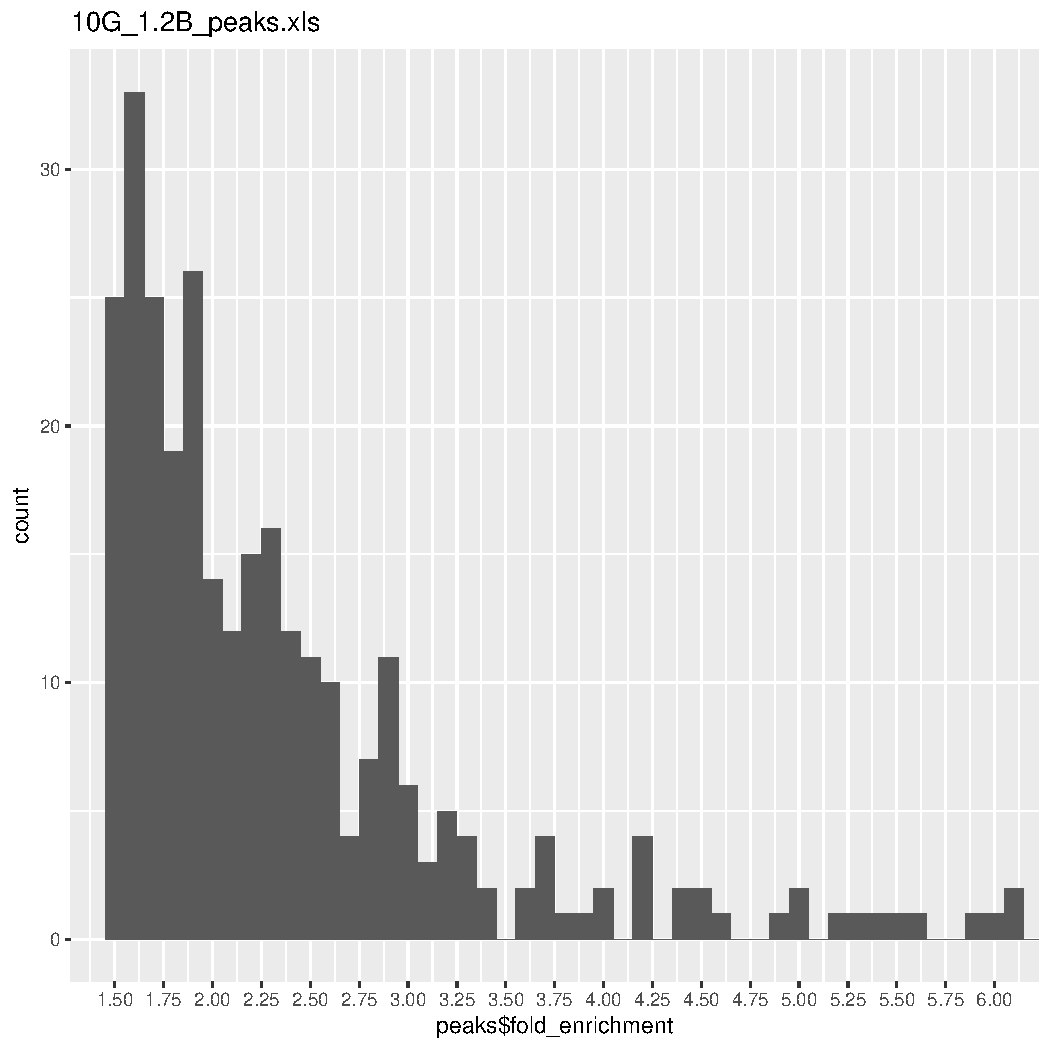
\includegraphics[width=\maxwidth]{figure/unnamed-chunk-2-1} 

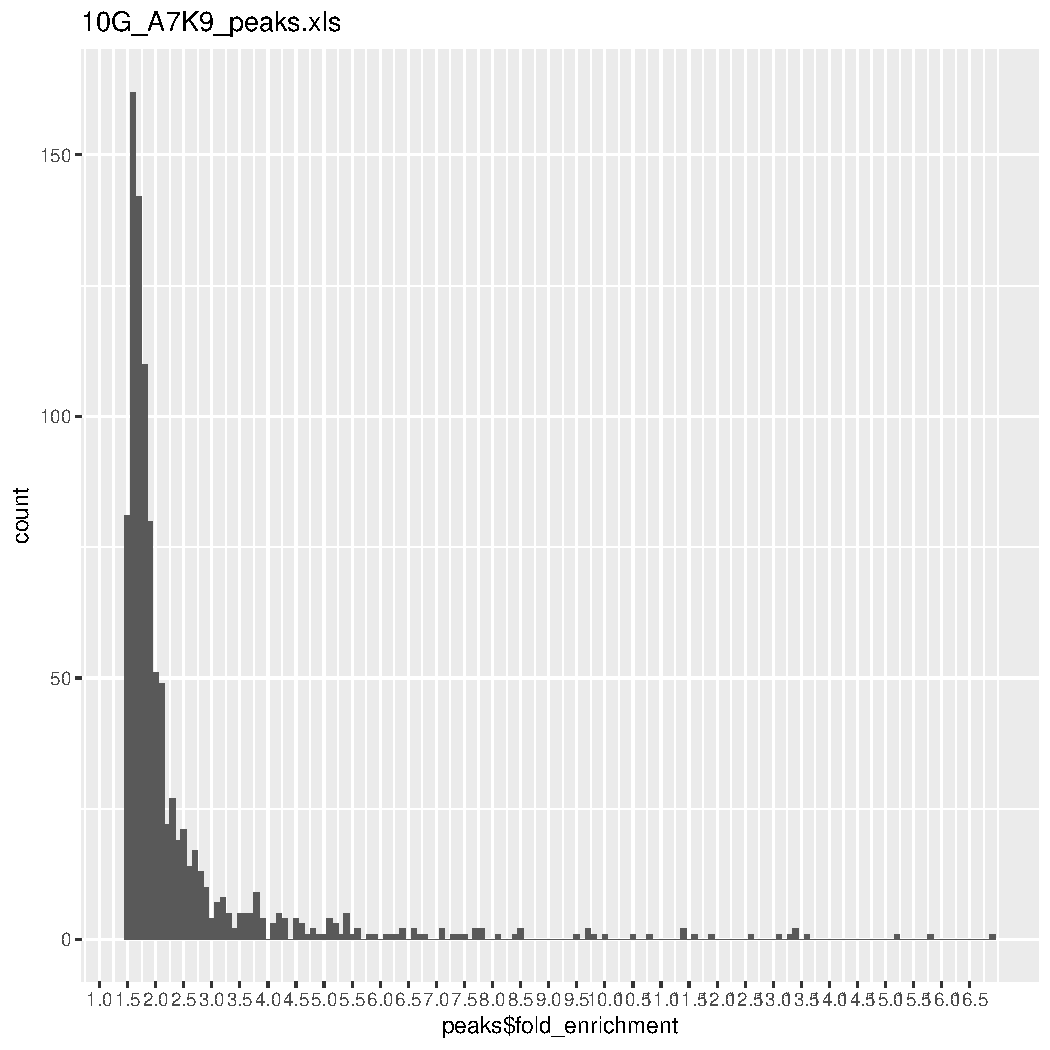
\includegraphics[width=\maxwidth]{figure/unnamed-chunk-2-2} 

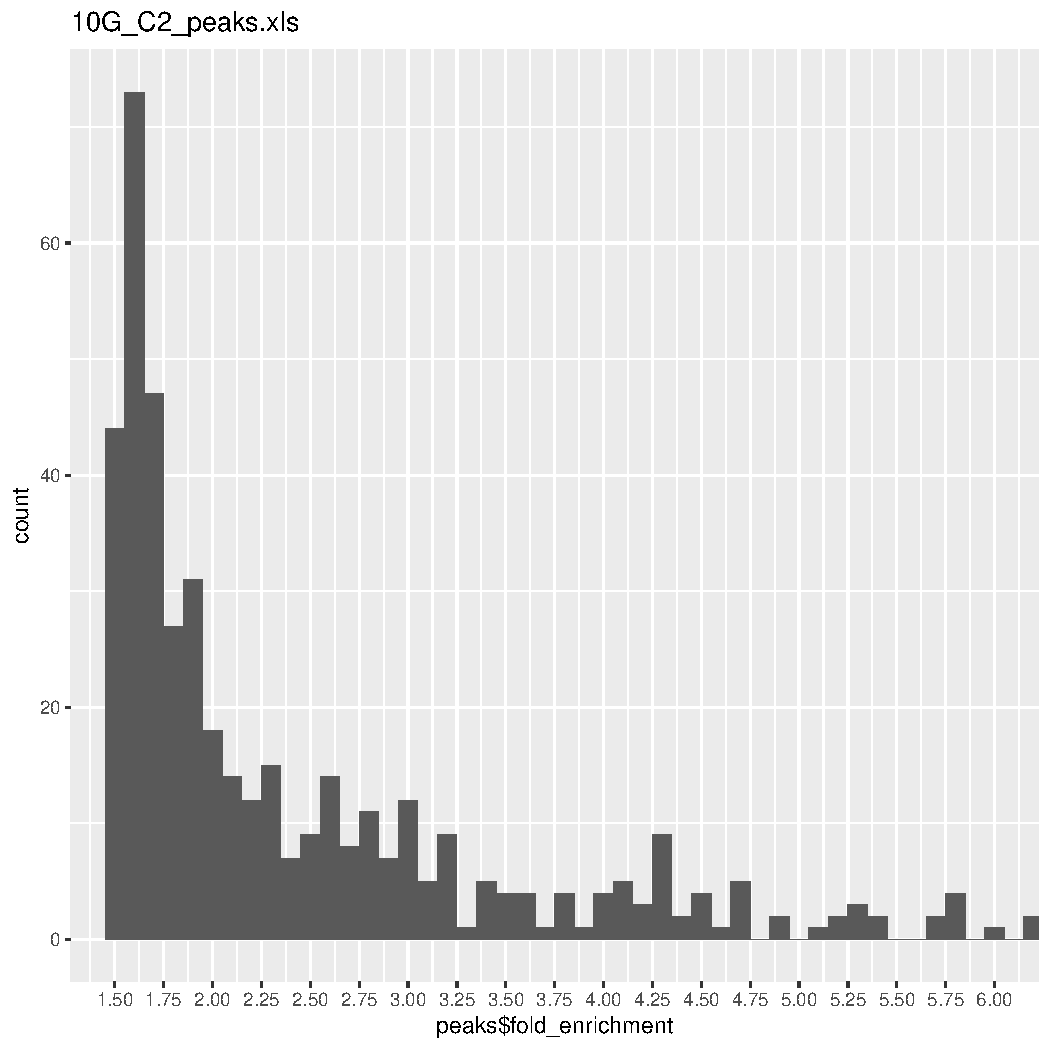
\includegraphics[width=\maxwidth]{figure/unnamed-chunk-2-3} 

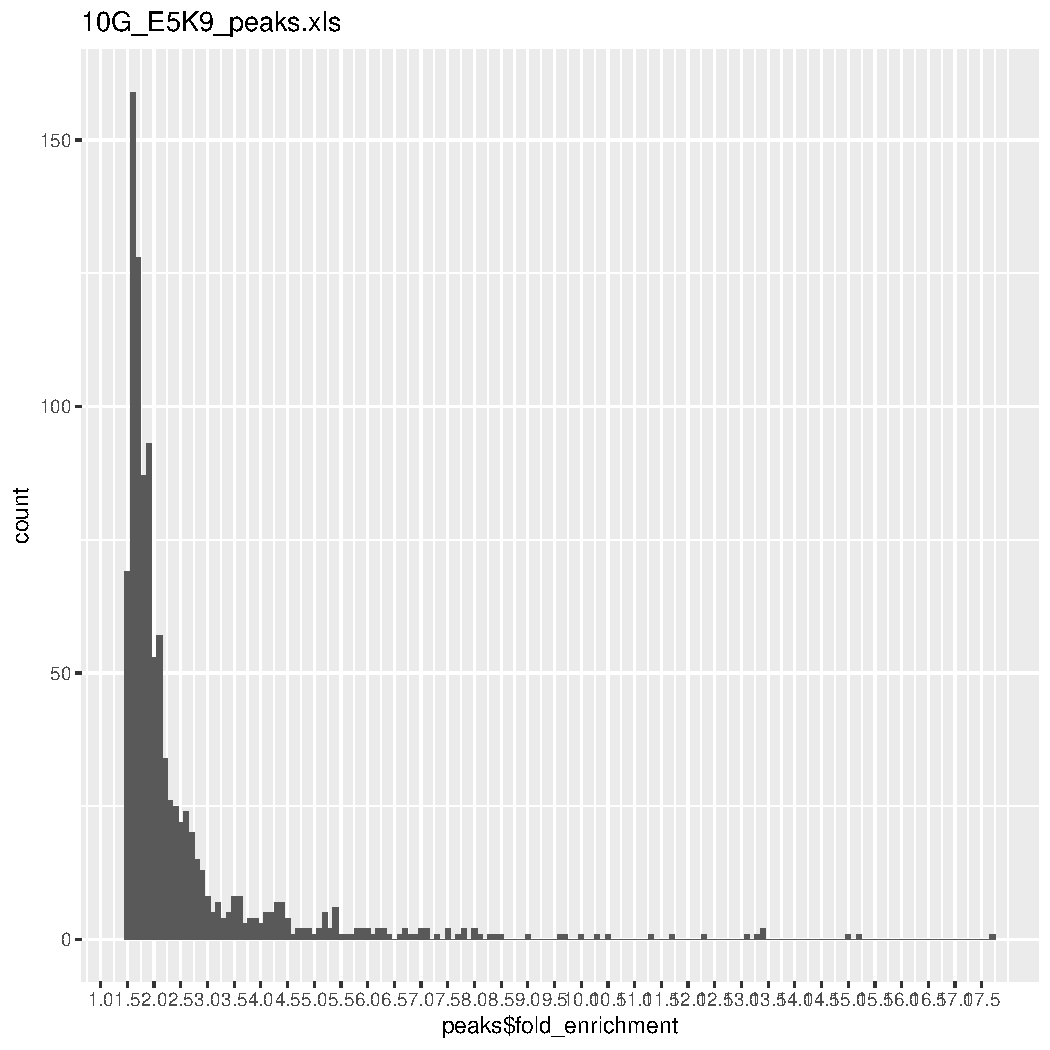
\includegraphics[width=\maxwidth]{figure/unnamed-chunk-2-4} 

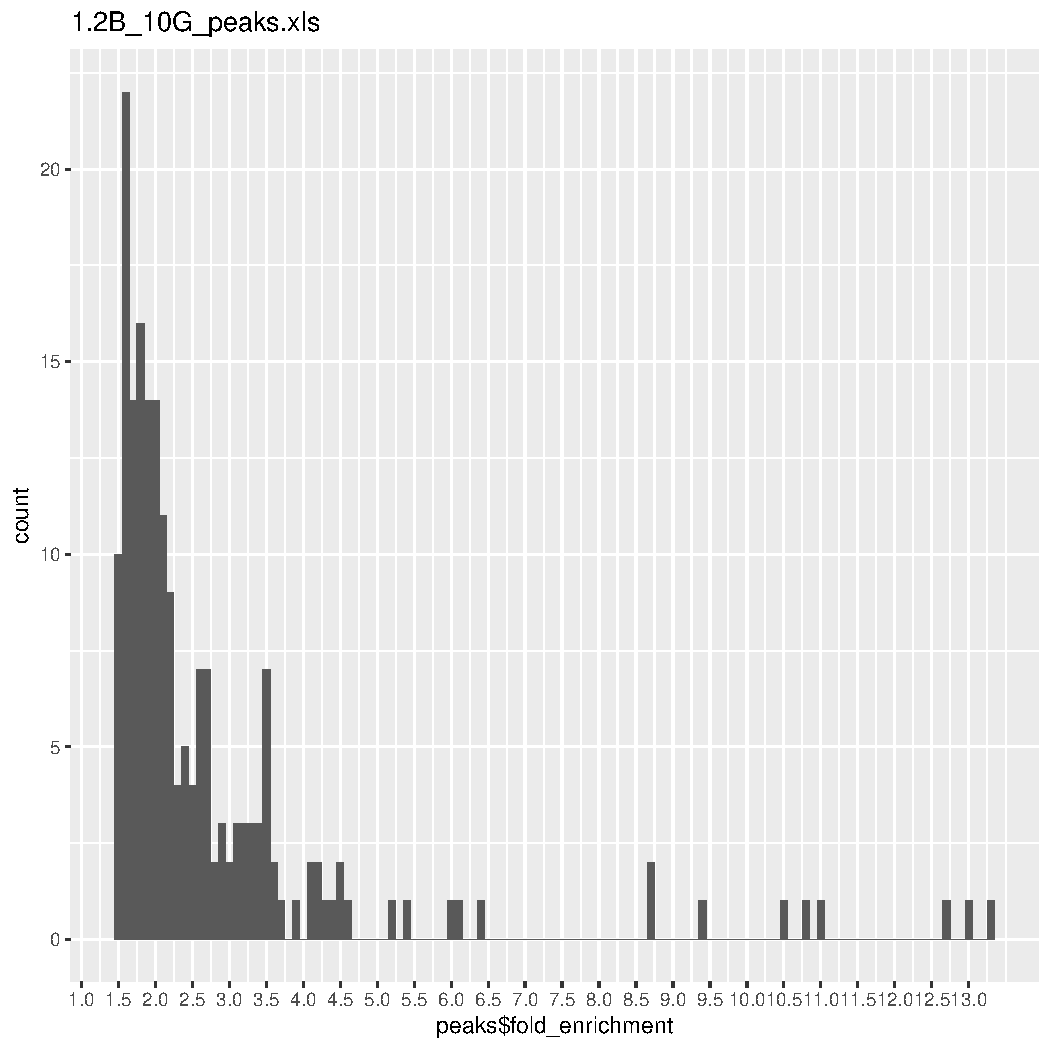
\includegraphics[width=\maxwidth]{figure/unnamed-chunk-2-5} 

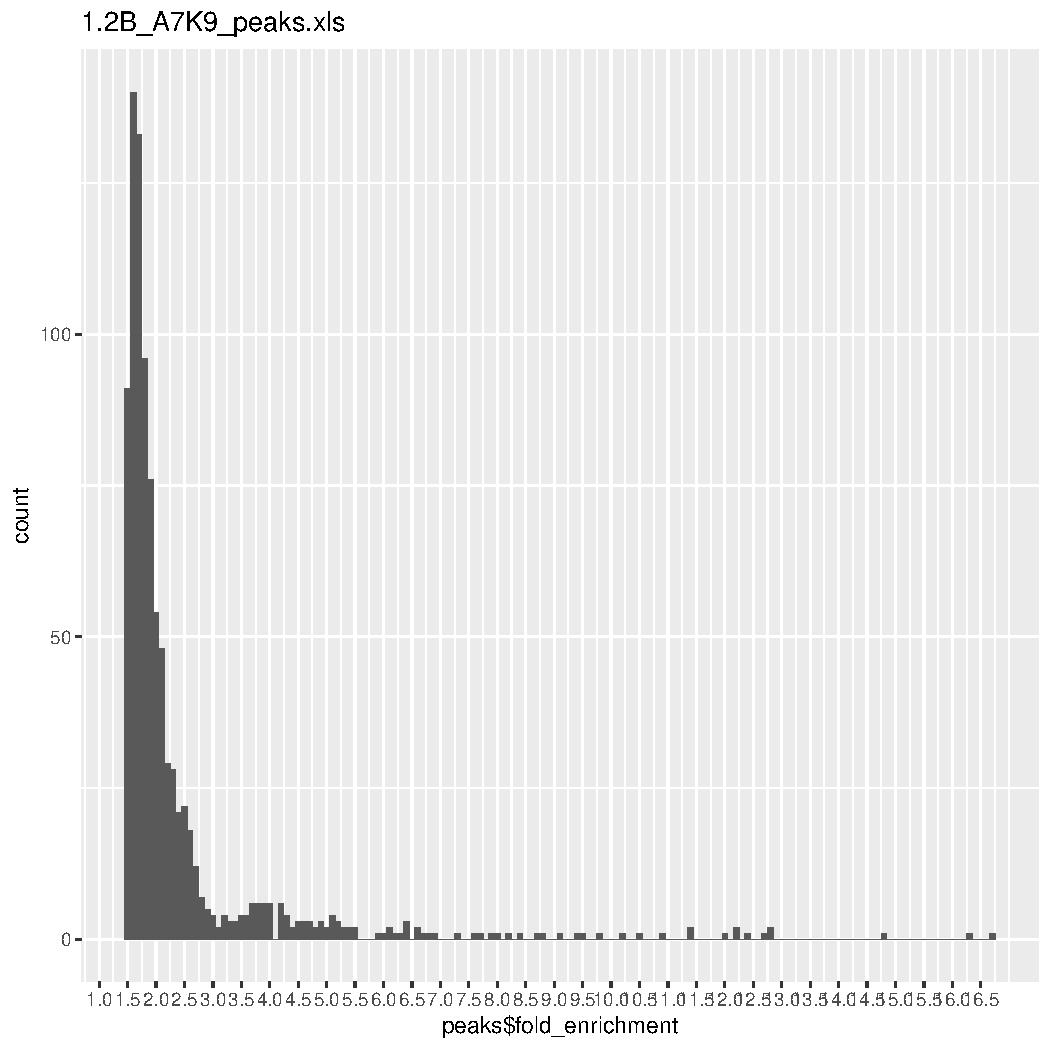
\includegraphics[width=\maxwidth]{figure/unnamed-chunk-2-6} 

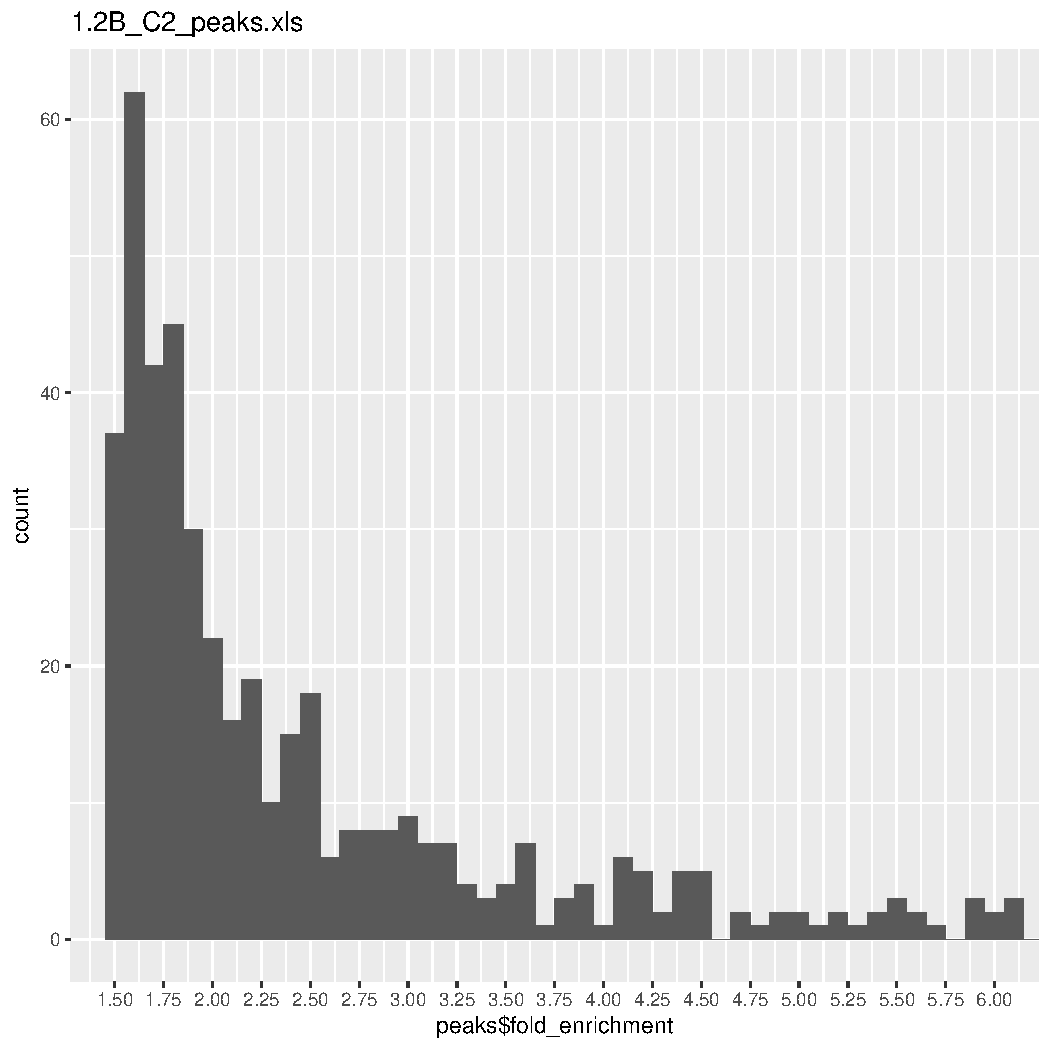
\includegraphics[width=\maxwidth]{figure/unnamed-chunk-2-7} 

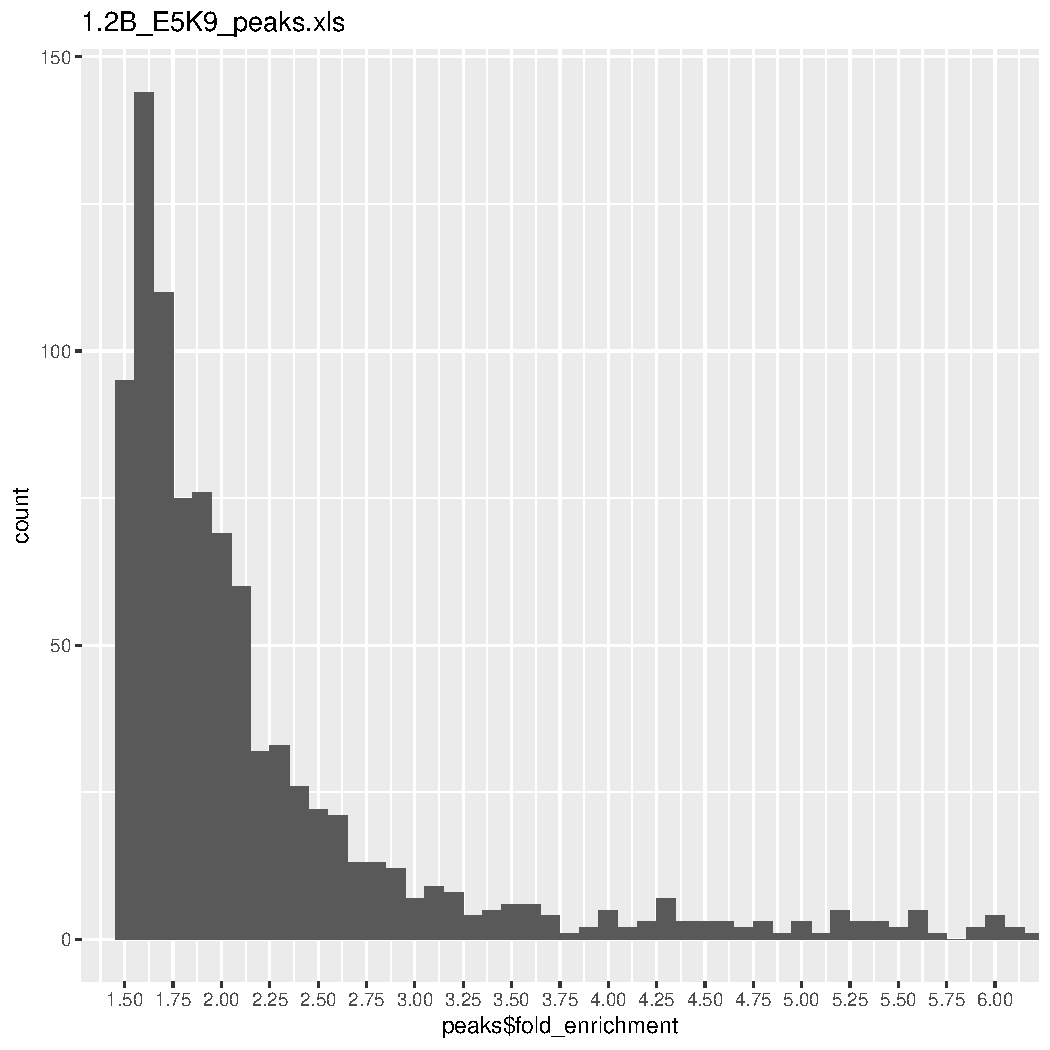
\includegraphics[width=\maxwidth]{figure/unnamed-chunk-2-8} 

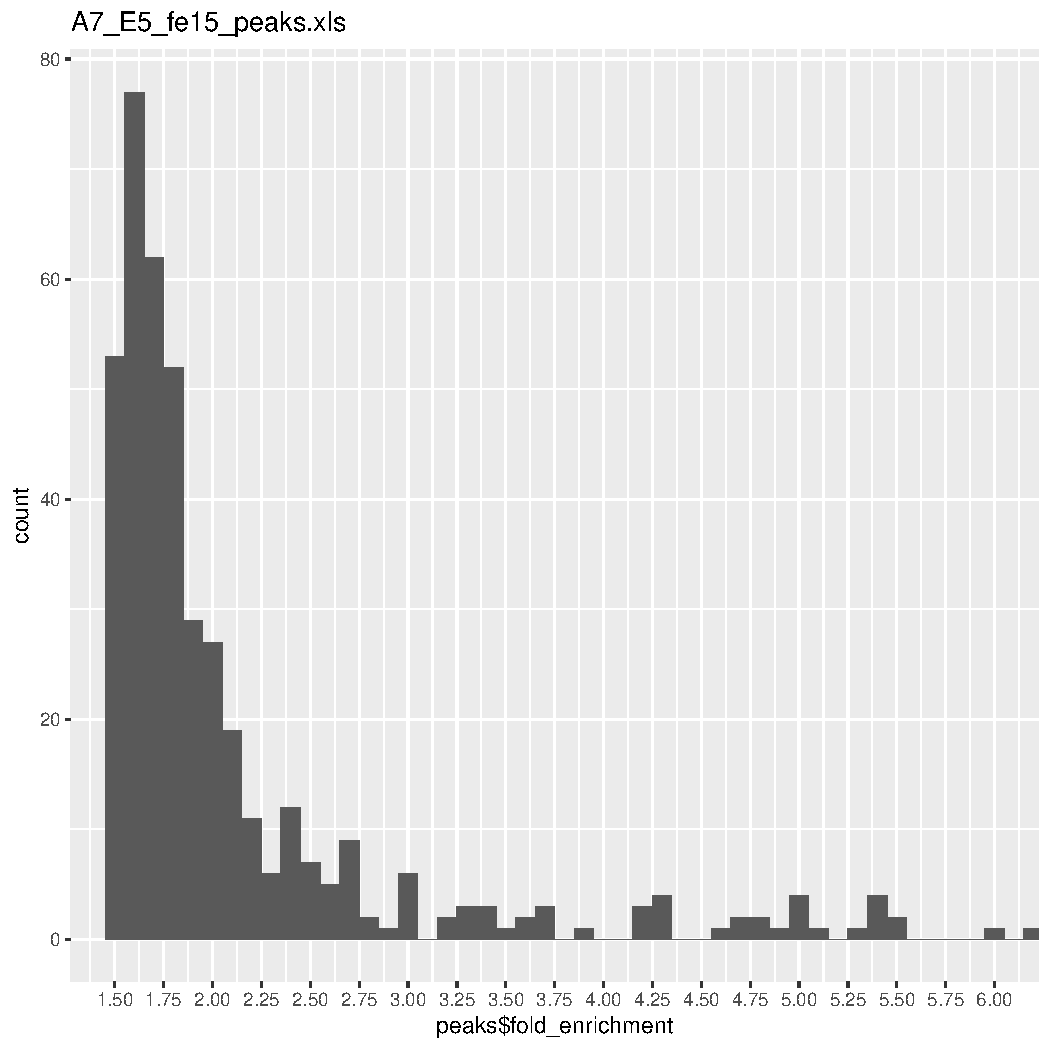
\includegraphics[width=\maxwidth]{figure/unnamed-chunk-2-9} 

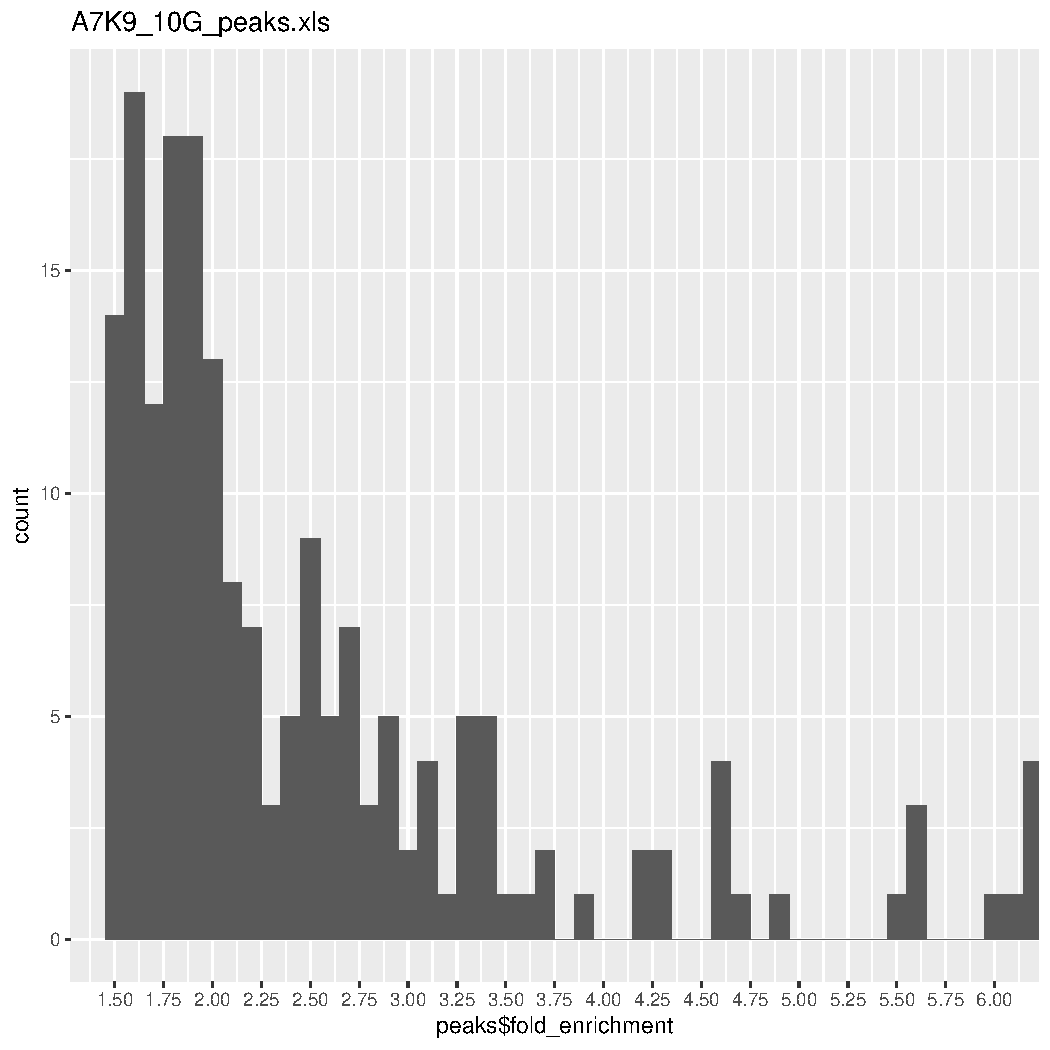
\includegraphics[width=\maxwidth]{figure/unnamed-chunk-2-10} 

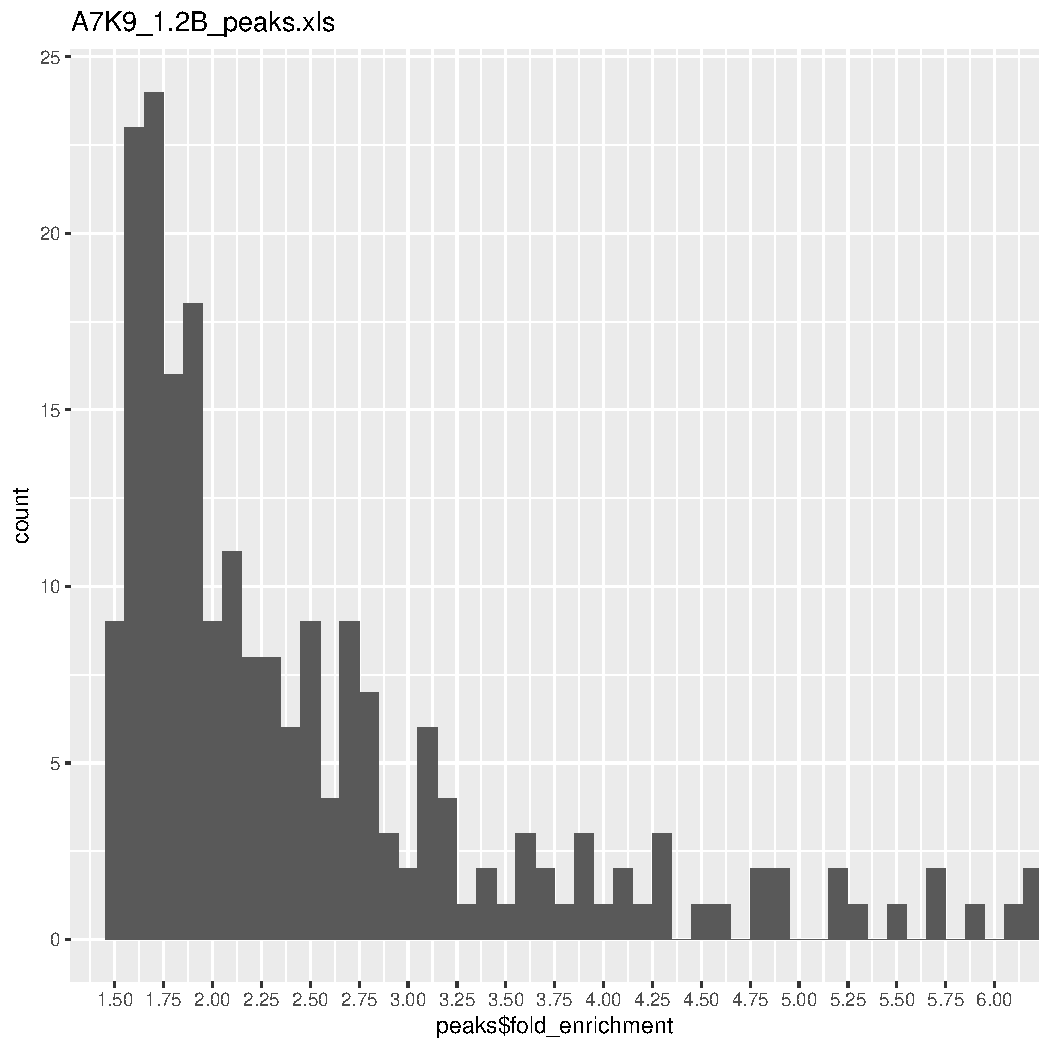
\includegraphics[width=\maxwidth]{figure/unnamed-chunk-2-11} 

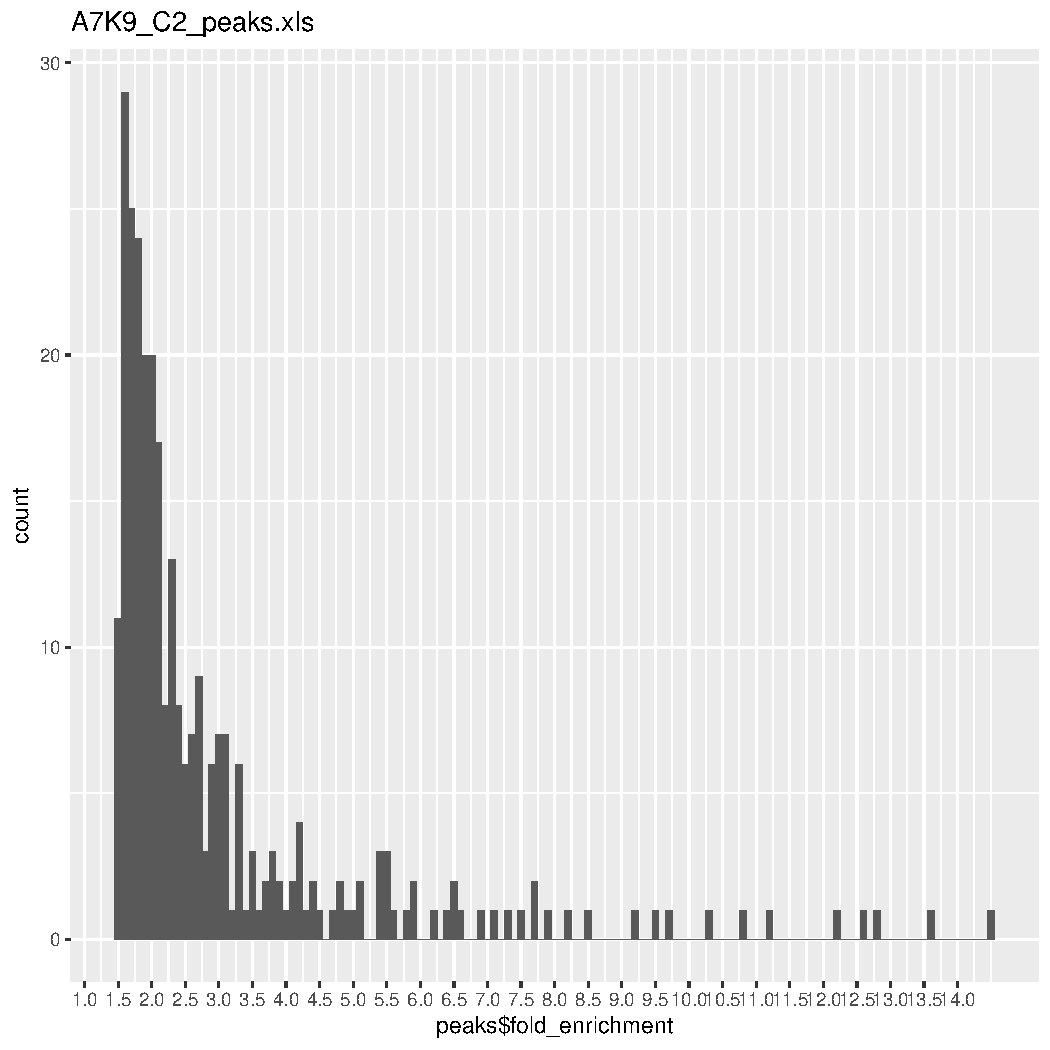
\includegraphics[width=\maxwidth]{figure/unnamed-chunk-2-12} 

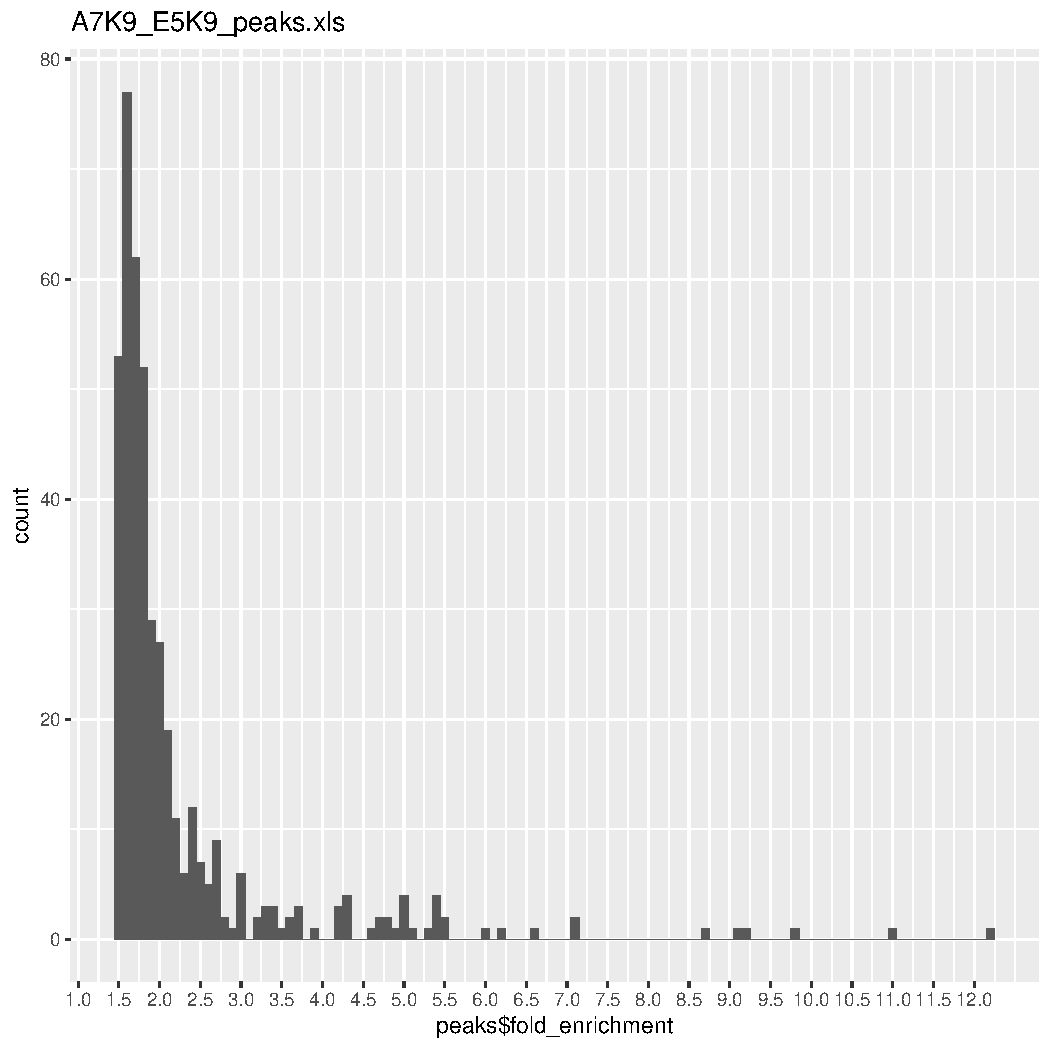
\includegraphics[width=\maxwidth]{figure/unnamed-chunk-2-13} 

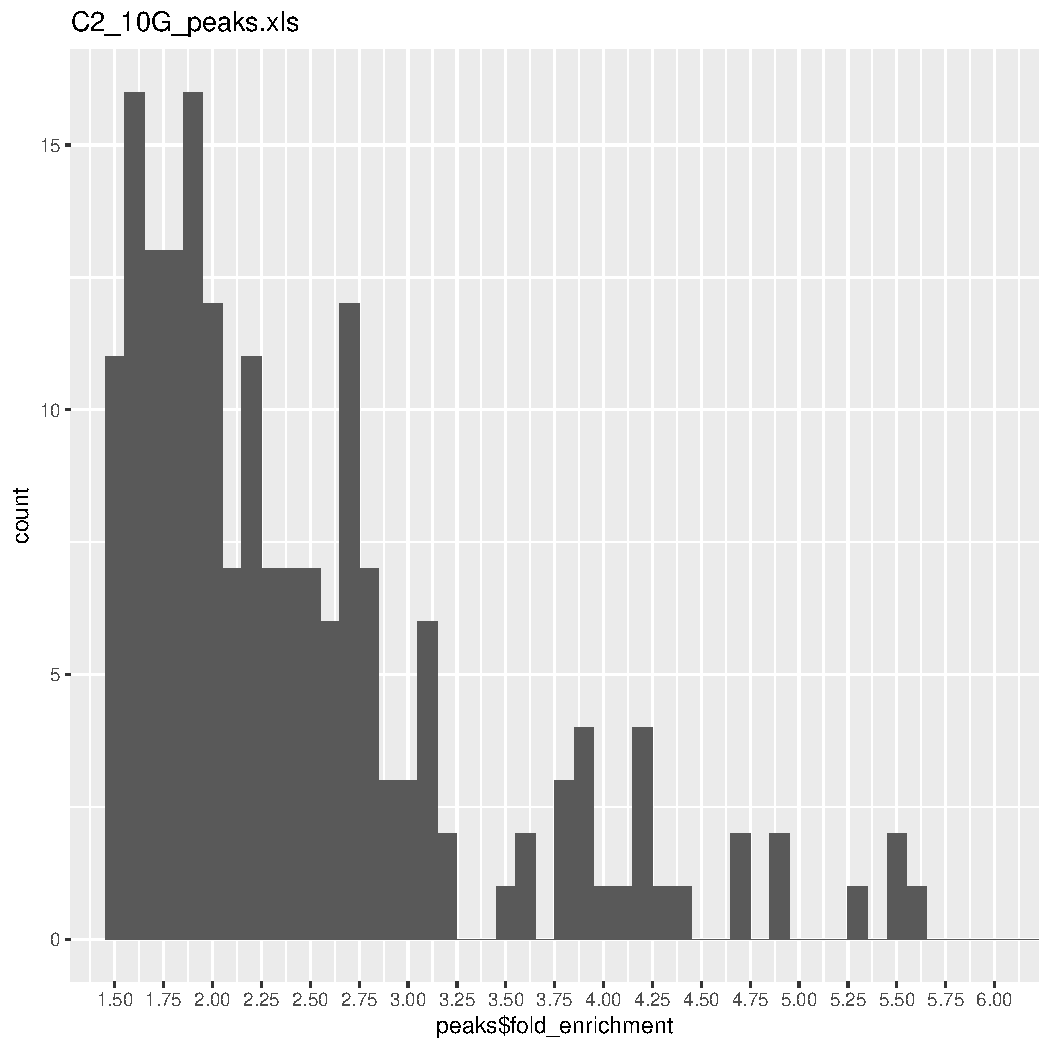
\includegraphics[width=\maxwidth]{figure/unnamed-chunk-2-14} 

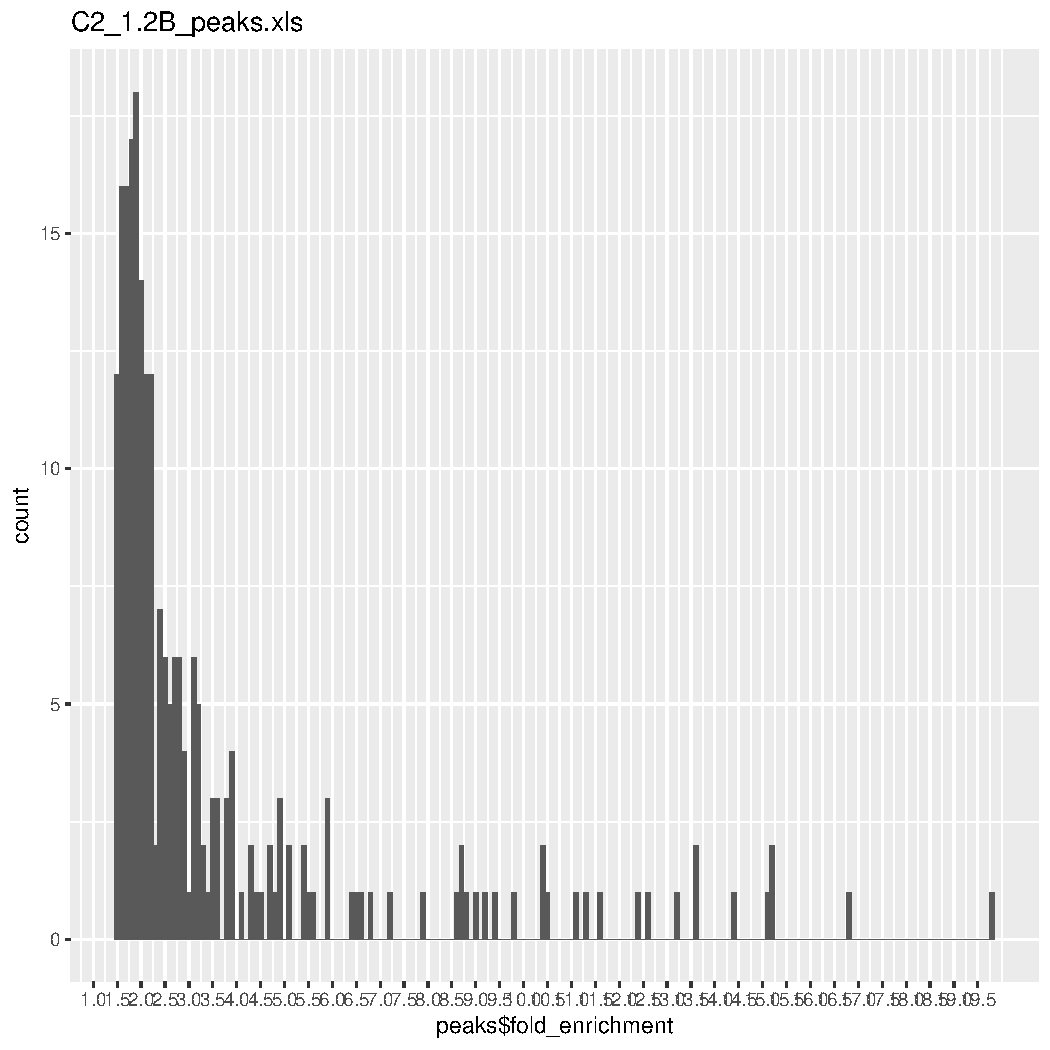
\includegraphics[width=\maxwidth]{figure/unnamed-chunk-2-15} 

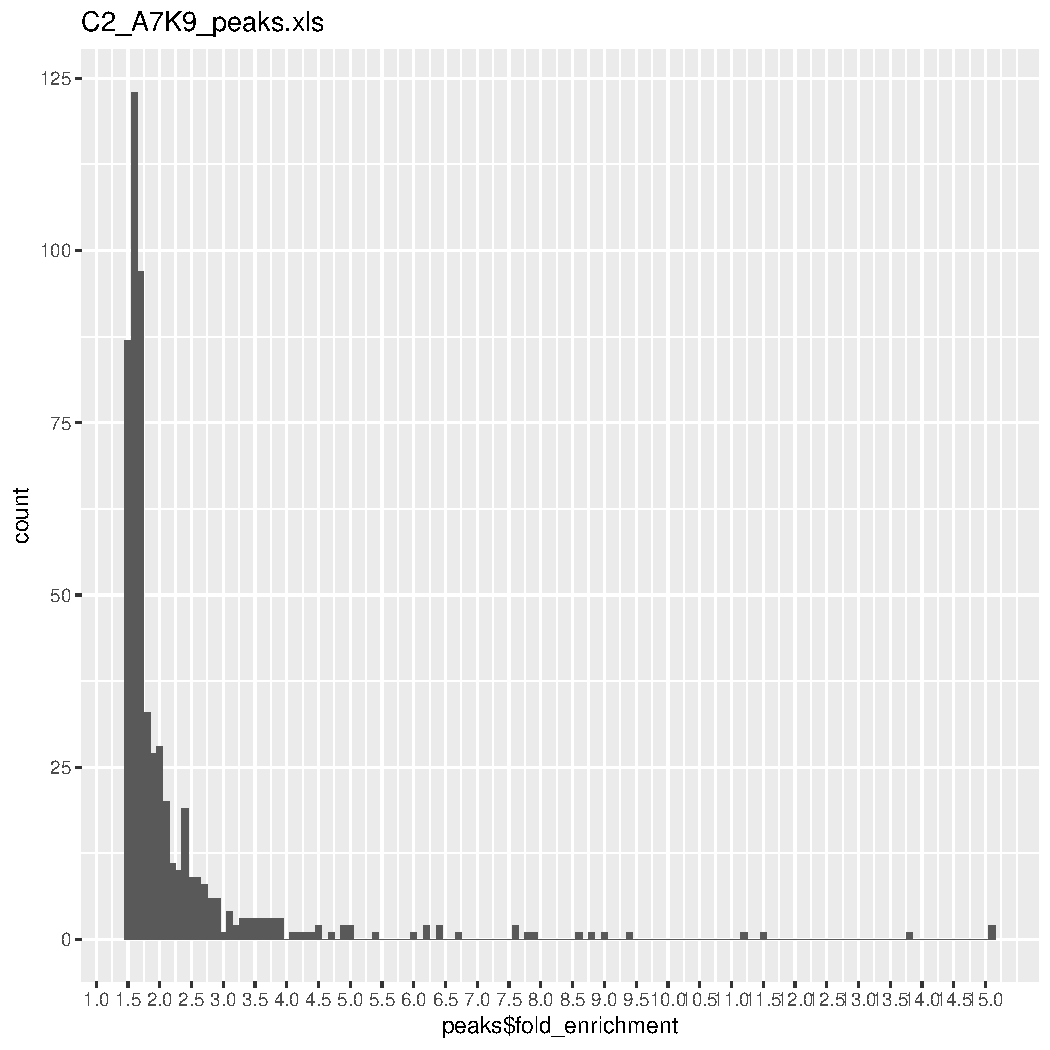
\includegraphics[width=\maxwidth]{figure/unnamed-chunk-2-16} 

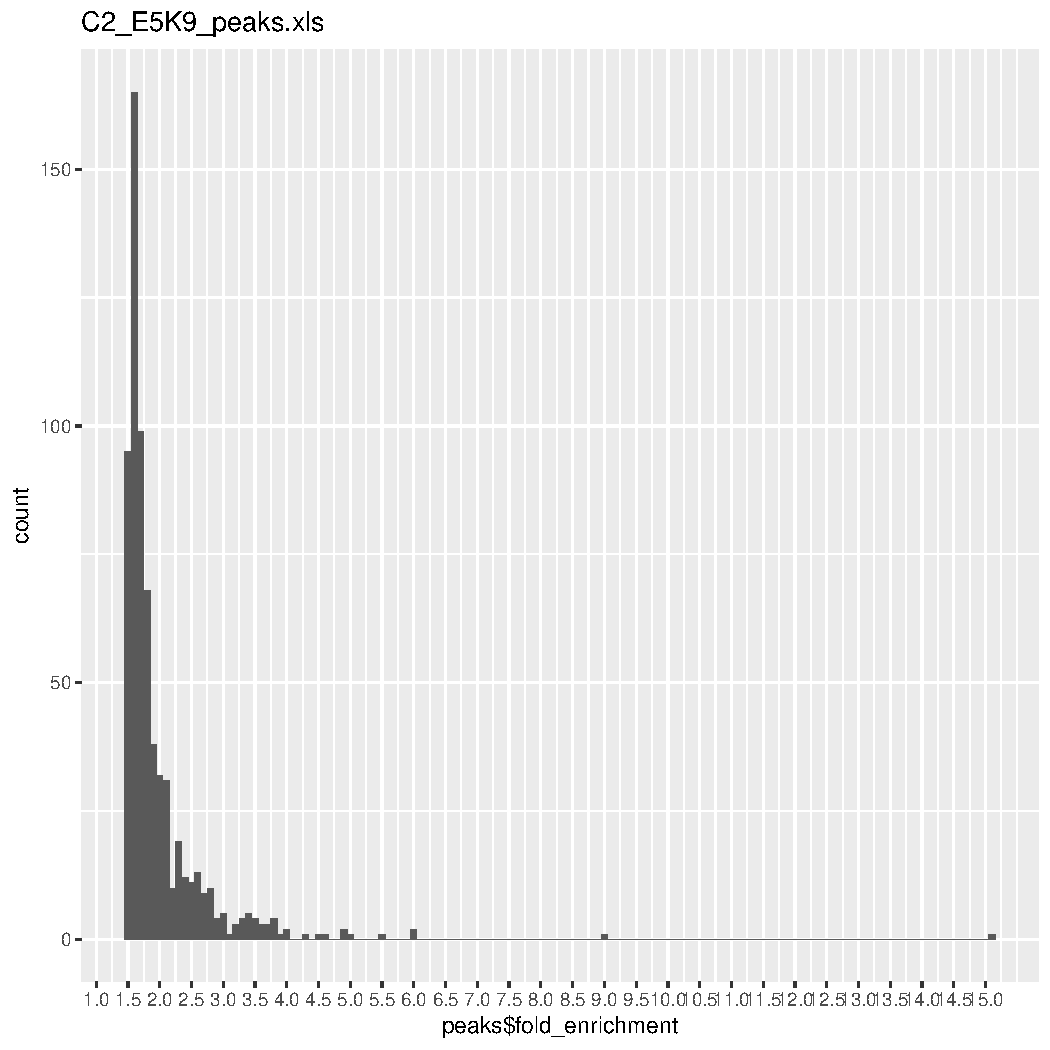
\includegraphics[width=\maxwidth]{figure/unnamed-chunk-2-17} 

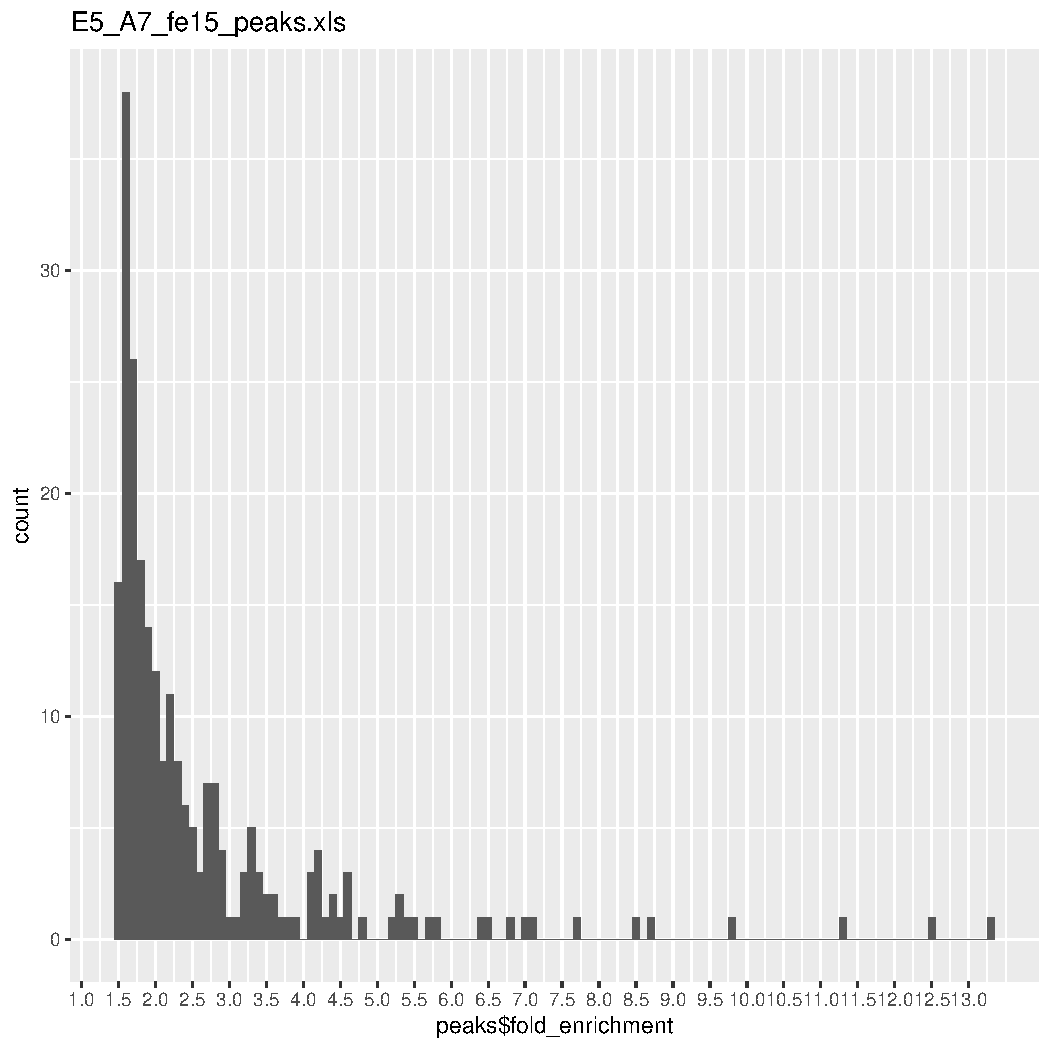
\includegraphics[width=\maxwidth]{figure/unnamed-chunk-2-18} 

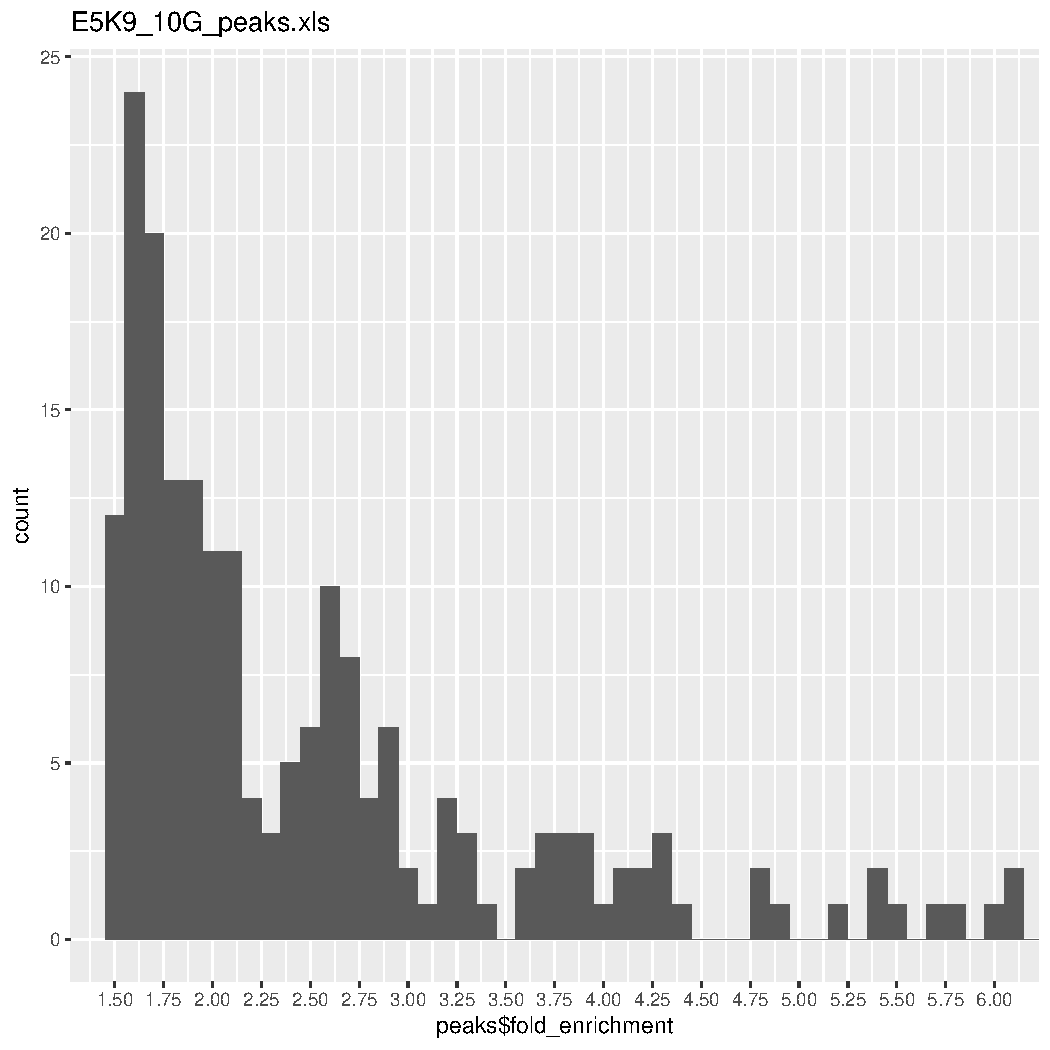
\includegraphics[width=\maxwidth]{figure/unnamed-chunk-2-19} 

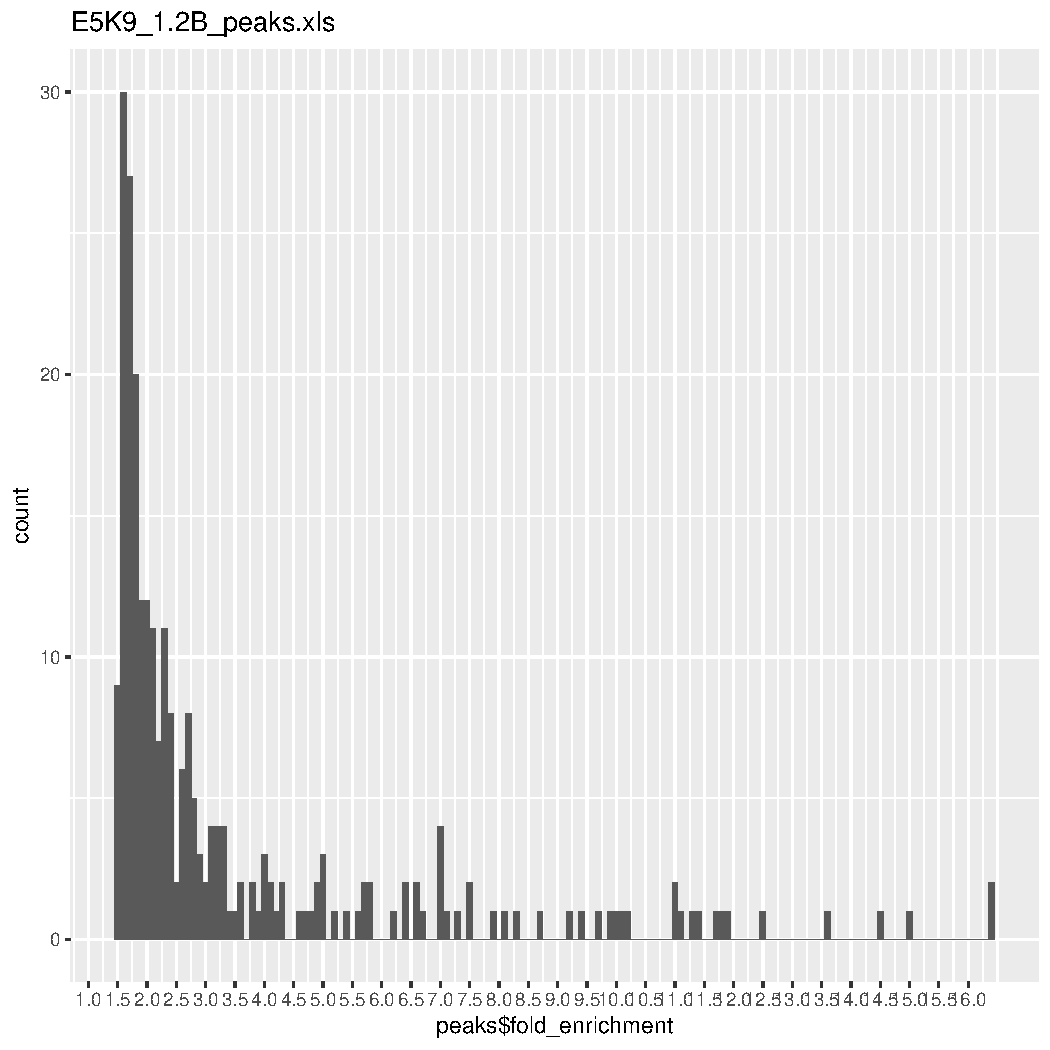
\includegraphics[width=\maxwidth]{figure/unnamed-chunk-2-20} 

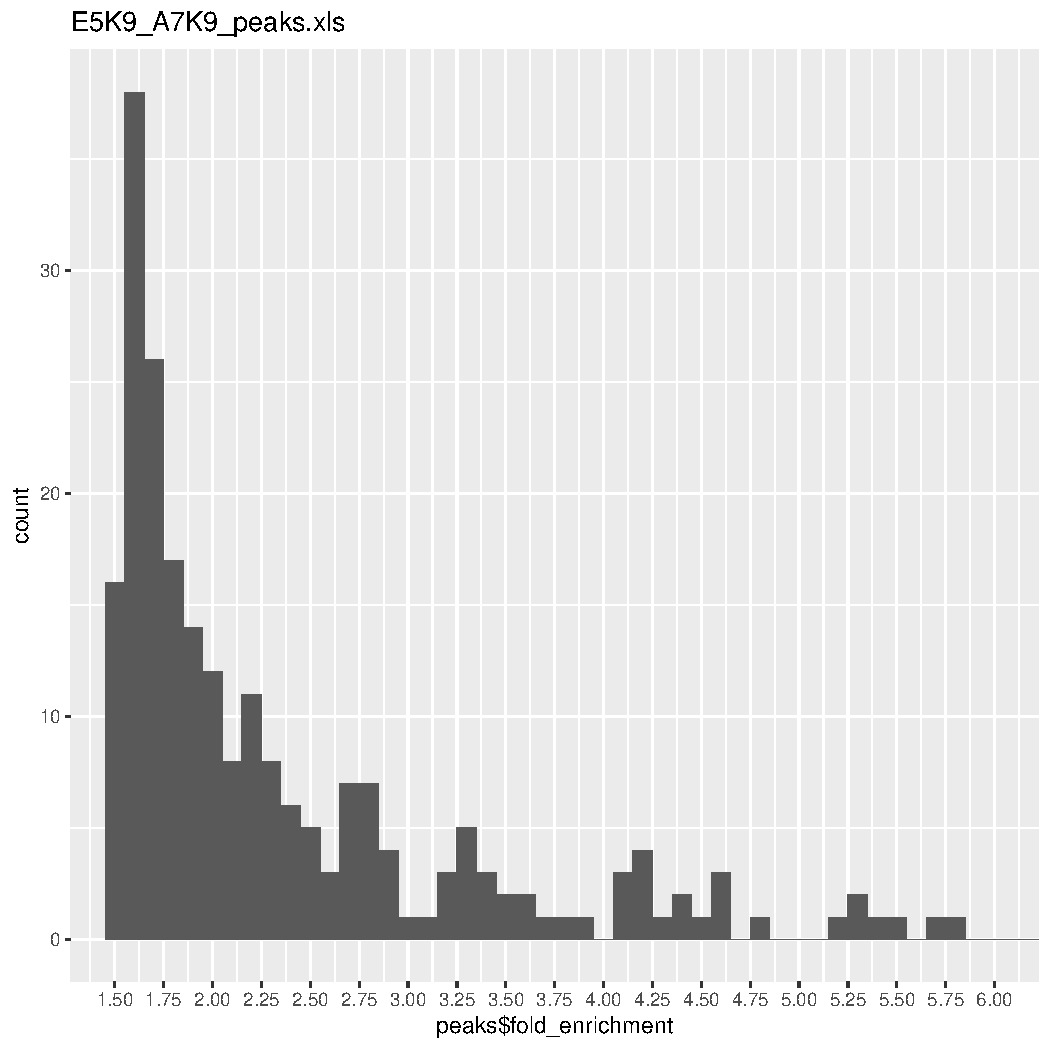
\includegraphics[width=\maxwidth]{figure/unnamed-chunk-2-21} 

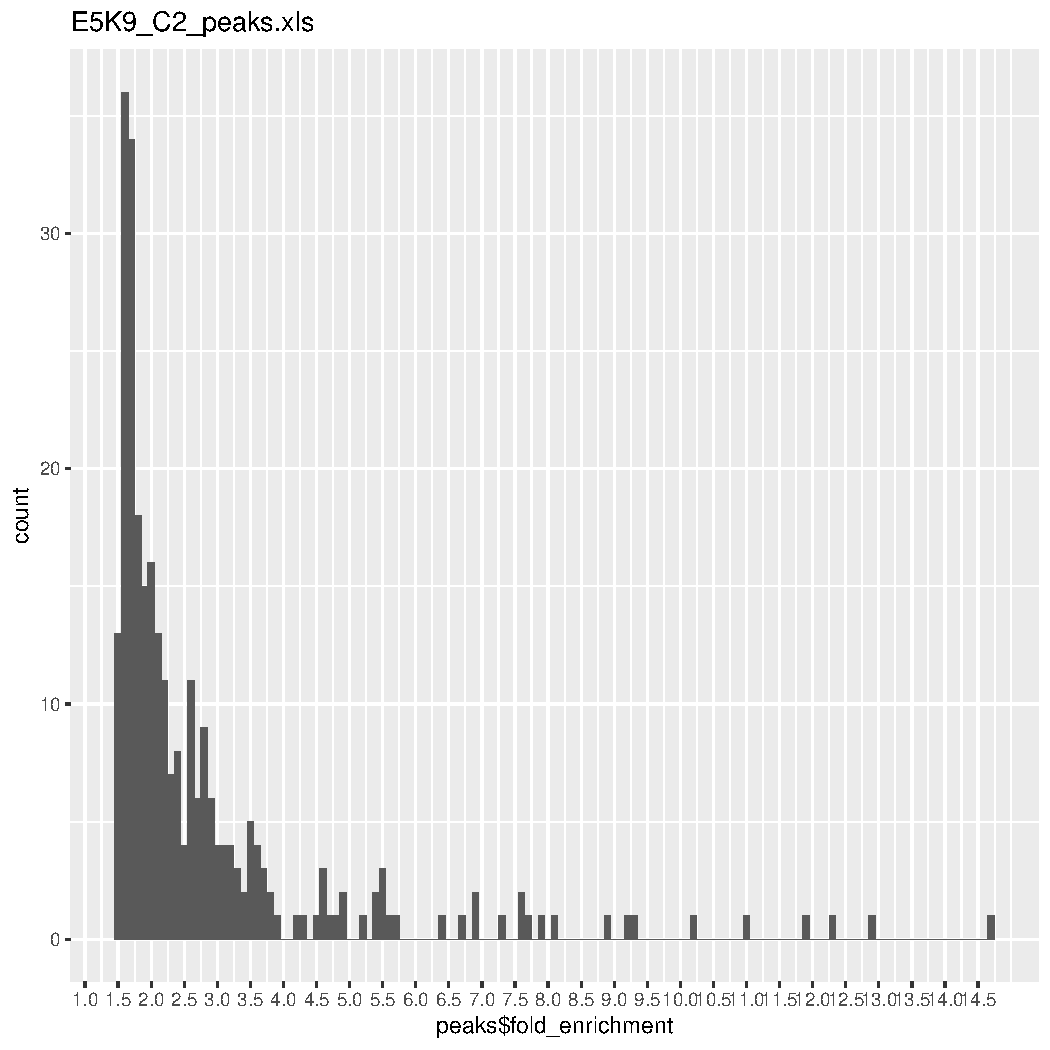
\includegraphics[width=\maxwidth]{figure/unnamed-chunk-2-22} 

\end{knitrout}


\end{document}
